% % % % % % % % % % % % % % % % 
\section{Work Plan}\label{chapterlabel4sec2}

These contributions demonstrate the potential value of a simulation system for advanced \ac{mri} sequences. 
Future work will focus on five areas:

%The PhD contributions so far demonstrate the value for an MRI simulation frame-work capable of producing realistic MRI datasets of advanced sequences in anaccurate and rapid manner. Future work will therefore include:

\begin{enumerate}
    % % % 
    %\item \textit{Write an MRI simulators review paper.}
    \item \textit{\textbf{An \ac{mri} simulators review paper} (first entry in Figure~\ref{fig:ganttChart})} \\
    So far, I have investigated the current state-of-the art in \ac{mri} simulation systems and experimented with 2 of the most popular and active \ac{mri} simulators today.
    It is my plan for the future work to focus on fleshing out the literature review of this thesis into a review paper.
    
    % % % 
	\item \textit{\textbf{Continue with motion-corrupted \ac{mrf} experiments} (second entry in Figure~\ref{fig:ganttChart})} \\
	So far, I have investigated how in-plane motion corrupts the \ac{mrf} quantitative maps.
	In the future, I aim to investigate through-plane motion and a combination of both in-plane and through-plane motion for the original \ac{mrf} implementation by Ma et al. \cite{Ma2013}.
	
	% % % 
	\item \textit{\textbf{Develop an open-source MRI simulator that will allow for the simulation of advanced MRI sequences} (third entry in Figure~\ref{fig:ganttChart})} \\
	
	So far, I have implemented a proof-of-concept simulation framework for an \ac{mrf}-\ac{bssfp} experiment in an open-source simulator called JEMRIS \cite{Stocker2010}.
	However, the newest implementation of an \ac{mrf} sequence relies on a \ac{fisp} type acquisition protocol for which a high number of isochromats is required in order to achieve realistic results.
	With the current JEMRIS implementation, this would require an unfeasibly long time to simulate.
	The reason for this is:
	
	\begin{itemize}
	    
	    \item I have calculated that a JEMRIS numerical simulation of a single voxel \ac{fisp} protocol that achieves the same results as the \ac{epg} implementation shown in Chapter \ref{method:fispdictionary} would require around 5000 isochromats. \\
	    
	    In my current implementation the input object consists of 4145 isochromats in total and requires a total time of 12 hours to run.
	    This means that in order to achieve accurate results I would need to discretise the input object to contain approximately 21 million isochromats.
	    This would bring the current simulation time to almost a year.
	    
	\end{itemize}
	
    % 	On the other hand, my own MATLAB simulations of a single voxel \ac{fisp} experiment show that I can achieve the same accuracy as an \ac{epg} implementation with approximately 200 isochromats.
	For this reason, it is my plan for future work to develop an open-source MRI simulator based on \ac{gpu} parallelisation and the newest programming standards offered by CUDA 9.x.
	The reasons for choosing \ac{gpu} parallelisation are:
	
	\begin{itemize}
	    
	    \item Xanthis et al. \cite{Xanthis2014} showed that their \ac{gpu}-based \ac{mri} simulation system can achieve a speedup of $31$ to $115$ times compared to OpenMP \ac{cpu} parallelisation.
	    However, their simulator is neither open-source, nor freely available to be downloaded and used.
	    
	    \item In their experiment they simulated a simple gradient echo sequence using an input object of $15 \times 15 \times 15cm$ consisting of $1, 350, 000$ isochromats (or, $400$ isochromats in every $cm^3$).
	    Their simulation took approximately $4.8$ minutes.
	    
	    \item My own MATLAB simulations of a single voxel \ac{fisp} experiment show that I can achieve the same accuracy as an \ac{epg} implementation with approximately 200 isochromats.
	    This means that I could bring down the simulation time to 40 hours by using the same experiment design as Xanthis et al. \cite{Xanthis2014}, but with $200$ isochromats in every $mm^3$ of a $15 \times 15 \times 15cm$ object and considering a linear increase in the simulation time.
	    Their implementation, however, is on a single board \ac{gpu} personal computer and it uses an older version of the CUDA \ac{api}.
	    
	\end{itemize}
	
	Implementing the open-source \ac{gpu}-based MRI simulator will consists of the following steps:
	\begin{enumerate}
	    
	    \item One voxel experiments:
	    \begin{itemize}
	        \item Develop a simple \ac{bssfp} experiment (single readout, multiple repetition periods) and compare it against my current MATLAB implementation.
	        
	        \item Develop a simple \ac{fisp} experiment (single readout, multiple repetition periods) compared it against my current MATLAB implementation.
	        
	        \item Experiment with different numbers of isochromats and find the critical number of spins required.
	    \end{itemize}
	    
	    \item Multiple voxel experiments:
	    \begin{itemize}
	        \item Develop a simple \ac{bssfp} experiment (EPI readout, one repetition period) and compare it against my current JEMRIS implementation.
	        
	        \item Develop a simple \ac{fisp} experiment (EPI readout, one repetition period) and compare it against my current JEMRIS implementation.
	        
	    \end{itemize}
	    
	    \item Develop the full \ac{mrf}-\ac{fisp} sequence.
	    
	\end{enumerate}	
	
	The general framework for my proposed simulation system is presented in the next section.
	In the remaining time of my PhD the focus will be on the development of a \ac{gpu}-based Bloch equation solver.
	
    % 	However, in order to mimic a continuous distribution of spins throughout an object voxel, a high number of isochromats is required to generate a smooth image intensity \cite{Shkarin1997}.
    % 	Moreover, newer \ac{mrf} implementations rely on an imaging sequence called fast imaging with steady state precession (\ac{fisp}, see Appendix \ref{MRIFISP}) which requires an even denser collection of spins to be accurate.
	
	\item \textit{\textbf{Validate the implementation} (fourth entry in Figure~\ref{fig:ganttChart})}
	So far, the simulation system has not been validated.
	This is because the real \ac{mrf} datasets that I have are for the \ac{mrf}-\ac{fisp} implementation.
	For this reason, I aim to demonstrate the applicability of my new simulator by validating it against real \ac{mrf}-\ac{fisp} datasets.
	
	\item \textit{\textbf{Simulate the impact of motion on the \ac{mrf}-\ac{fisp} sequence} (fifth entry in Figure~\ref{fig:ganttChart})}
	After validation, I will be in a great place to investigate the impact of motion on the \ac{mrf}-\ac{fisp} sequence.
	For this, I aim to look at in-plane, through-plane and a combination of both in-plane and through-plane motion for the newly developed simulation system.
	
\end{enumerate}

\begin{figure}[ht]
    \centering
    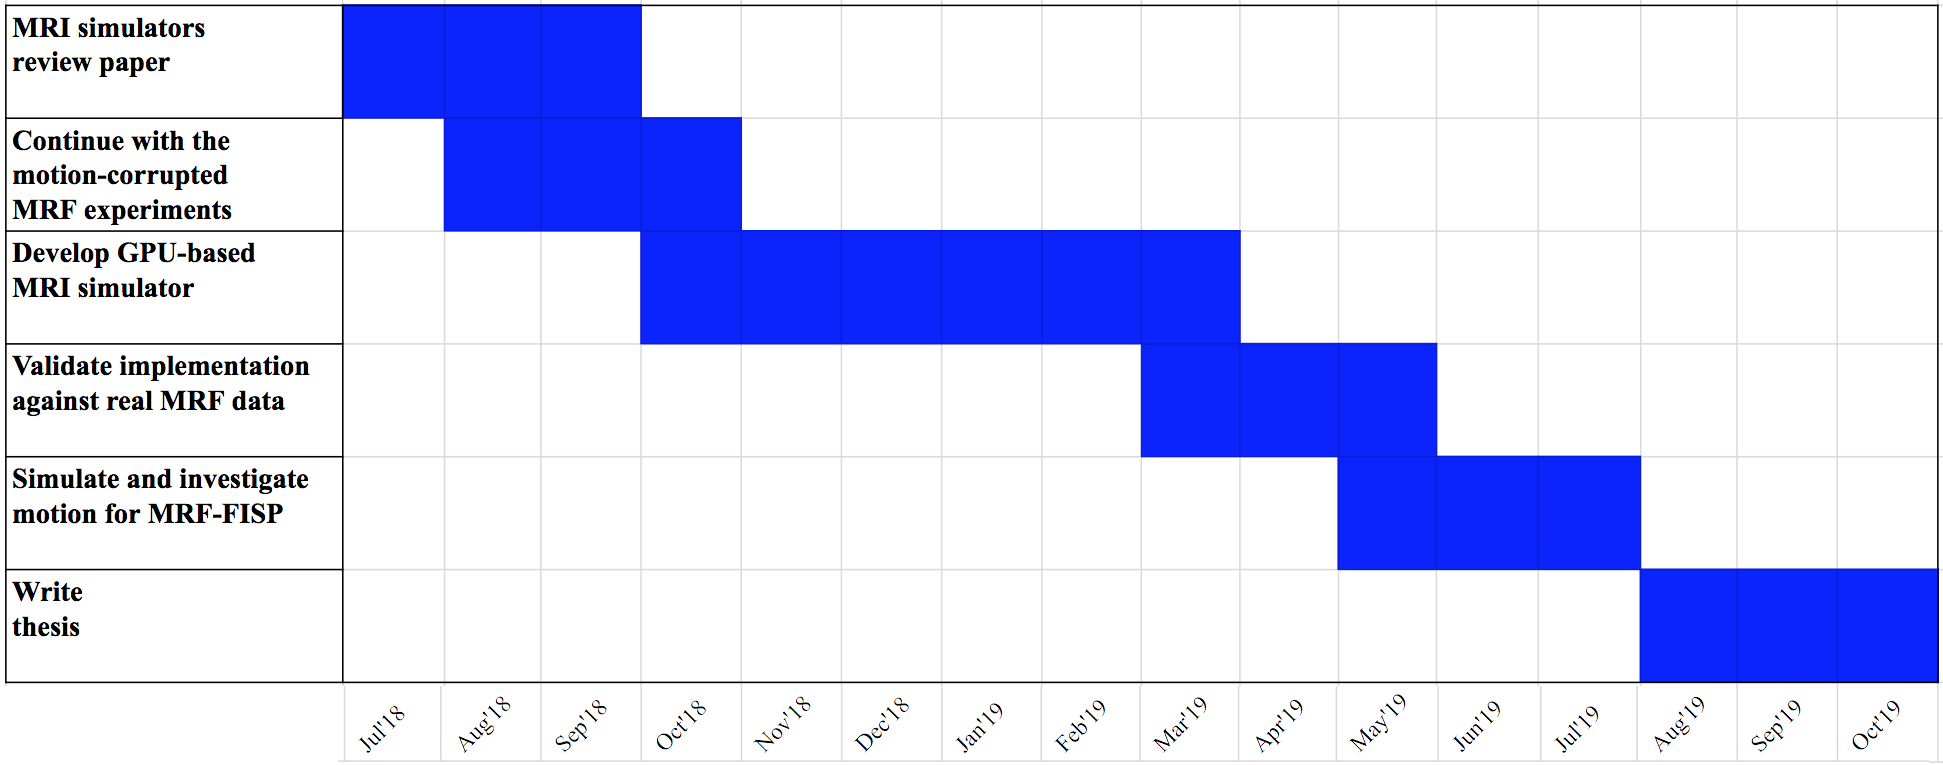
\includegraphics[width=1\textwidth, keepaspectratio]{images/mri/ganttChart}
    \caption{Gantt chart demonstrating how I will spend the remaining time in my PhD}
    \label{fig:ganttChart}
\end{figure}
